\section{Component View}


This section details the internal modules used in each component seen previously.
<<<<<<< HEAD
In particular, we focus on the main subcomponents of the business logic layer, as described in the previous chapter concerning the architecture overview. 
This because the main functionalities  of our software are almost all exploited at this level, whereas the other layer's components are mainly
=======
in particular, we focus about the main subcomponents of the business logic layer, as described in the previous chapter concerning the architecture overview. 
this because the main functionalities  of our software are almost all exploited at this level, whereas the other layer's components are mainly
>>>>>>> ad258dd7c9a37861a484c05c0be22fc9761a519f
designed in order to guarantee non functional features such as scalability or security. 

At component level, the software can be divided betweeen \emph{front-end components} and \emph{back-end components}; as a five-layers architecture, the \emph{Travlendar+} frontend is mainly represented by the client layer, which, as described in the \emph{Requirement analysis and specification document}, will be implemented as a mobile application and as web application, usable via browser.
\subsection{Front-end system}
<<<<<<< HEAD
In this subsection we mainly focus on the analysis of a possible generic client application, which can be implemented as a native application but also as a browser-oriented front-end.
Nowadays it is relatively simple to develop javascript based applications which uses web-oriented technologies without having to deal with common web browsers. this is the reason why is
natural to describe the two client interfaces using a single component diagram: the overall structure is similar, and the main differences are implementation related and thus not
=======
In this subsection we mainly focus on the analysis of a possible generic client application, which can be implemented as a native application but also as a browser-oriented frontend.
Nowadays it is relatively simple to develop javascript based applications which uses web-oriented technologies without having to deal with common web browsers. this is the reason why is
natural to describe the two client interfaces using a single component diagram: the overall structure is mainly similar, and the main differences are implementation related and thus not
>>>>>>> ad258dd7c9a37861a484c05c0be22fc9761a519f
discussed in this document.
\begin{figure}[H]
    \centering
    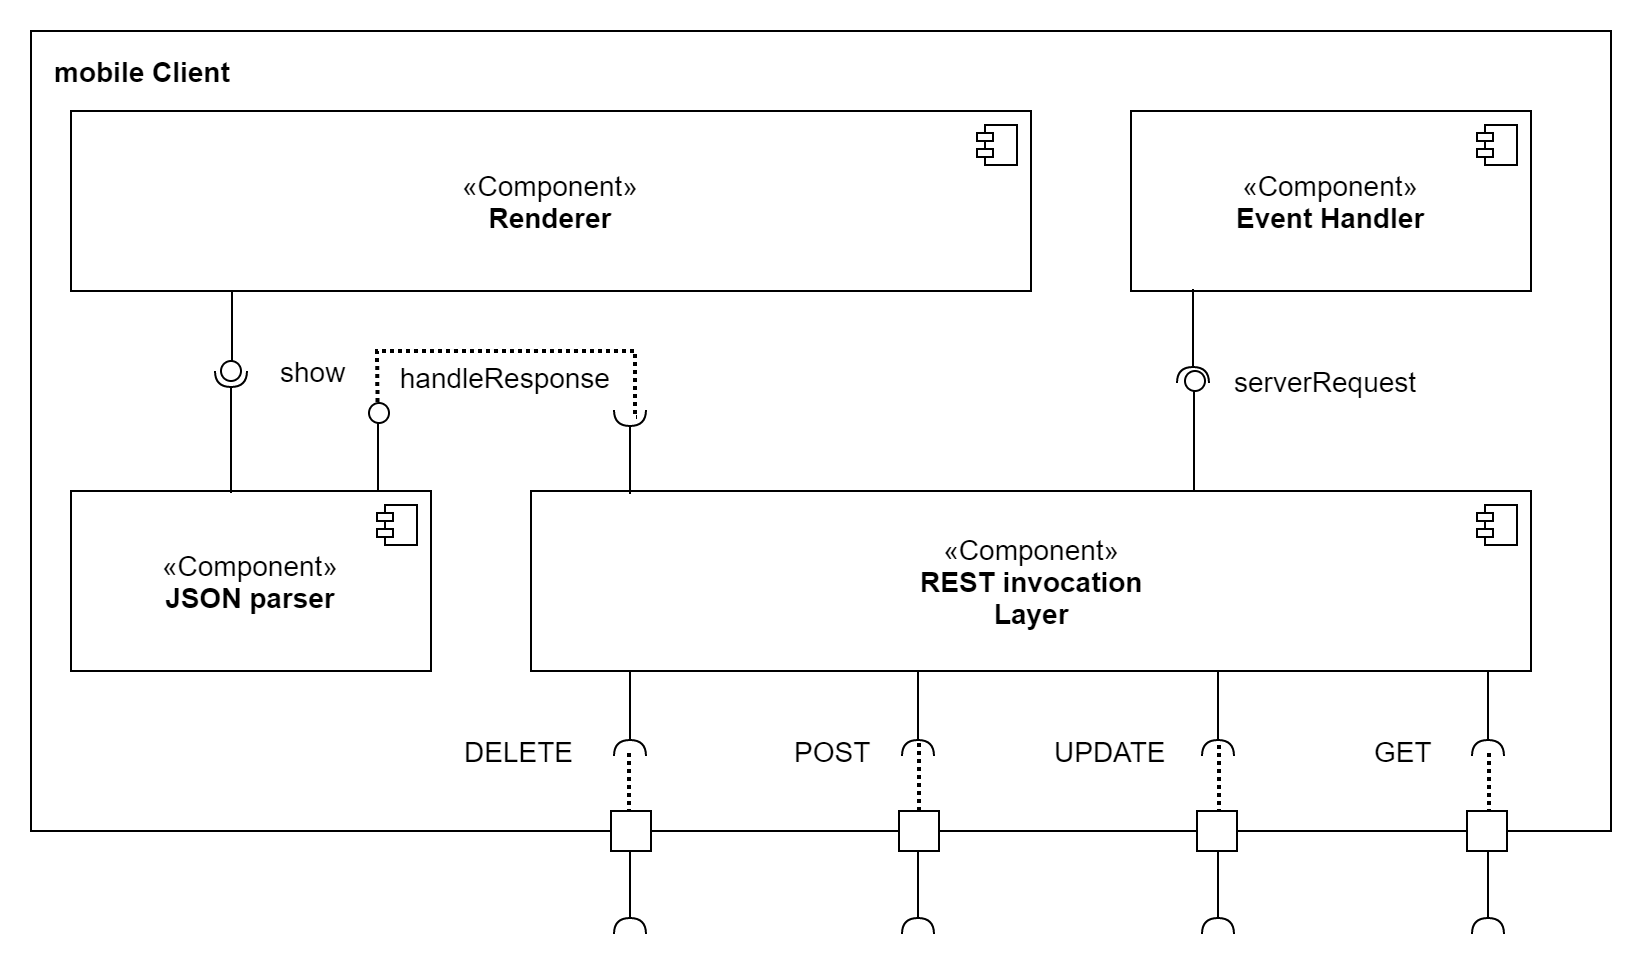
\includegraphics[scale=0.2]{Pictures/ComponentDiagram/client_component.png}
    \caption{UML component diagram about front-end components}
    \label{component:client}
\end{figure}

As seen in Figure \ref{component:client}, the main components are:
\begin{itemize}
<<<<<<< HEAD
    \item \textbf{the Renderer}: this component is meant to show data from the back end and display the interface from whom the user interacts with the application.
                                 in particular, the renderer is designed to be observed by other components, as in a traditional \emph{observable - observer pattern}:
                                 this choice has been made in order to make the renderer as much indipendent as possible with respect to the overall application, and
                                 vice versa, thus permitting to completely rewrite both the renderer and the application without modifying the other. 
                    
    \item \textbf{the JSON parser}: this component is meant to correctly interpret objects from server, so that the renderer can receive data without having to deal
                                    with the technologies used in other components. in particular, this component will receive JSON objects, it will interpret them and
                                    then call the correct functions from the renderer in order to populate the user interface.
                                    
    \item \textbf{the event handler}: this component will handle user imputs and call the network interface consequently. in particular, as seen when dealing about the 
                                      renderer, the \emph{observable - observer} approach will be used, so that the event handler \emph{observates} the graphical objects
                                      representation inside the renderer, and response in a proper way when a certain event is thrown.
                        
    \item \textbf{the REST invocation layer}: this component will handle the communication with the back-end. because of the chosen client-server approach, the front-end
                                              will mainly communicate with the back end using requests that are followed by proper responses. that is the reason why it is 
                                              simple to design the communication between the client and the server using HTTPS and REST requests. the responses will then 
                                              handled by the JSON parser, which will also update the graphic interface.
=======
    \item \textbf{the Renderer}: this component is meant to show datas from the back end and display the interface from whom the user interacts whith the application.
                                 in particular, the renderer is designed to be observed by other components, as in a traditional \emph{observable - observer pattern}:
                                 this choice has been made in order to make the renderer as much indipendent as possible with respect to the overrall application, and
                                 vice versa, thus permitting to  
    \item \textbf{the JSON parser}
    \item \textbf{the event handler}
    \item \textbf{the REST invocation layer}:
>>>>>>> ad258dd7c9a37861a484c05c0be22fc9761a519f
\end{itemize}


\subsection{Back-end system}
<<<<<<< HEAD
As claimed previously, the server software architecture is fairly more complex than the client software. the main reasons about this unbalance are simple:
\begin{itemize}
    \item the client hosts only the front-end, without operating any kind of business logic functionality.
    \item the back-end is built over three physical tiers, mainly for security and scalability reasons.
    \item the main idea between the back-end architectural design is to guarantee maintainability: all the software components will have to be as much as 
          modular and indipendent as possible, thus requiring to design proper adapters between components that certainly increases the overral complexity.
\end{itemize}

further informations about this choice regarding the physical architecture will be presented in the chapter regarding the deployment view, leaving this section
discuss only about how the software architecture is designed a priori. \\

\textbf{the Application Façade} 
        is a macro component that handles client requests and submit them to the application logic in a proper way. this component is required because
        of the choice to rely on HTTPS when dealing about the communication between front-end and back-end: it is then necessary a \emph{web server} component who handles
        rest request, and also an \emph{internal communication layer} who deals about translating https requests in TCP messages to be sent to the business logic components.
        this approach is preferable instead of permitting to the front end to directly send request to the business logic in order to avoid misuses. \\
        
\textbf{the Presenter layer}
        is the macro component which is in charge of receiving TCP messages from the application Façade and calling the business logic layer in order to satisfy the request. it is so mandatory to define a \emph{communication interface} component that mantains an open socket connection with the application Façade. the other two components we decided to define are:
        \begin{itemize}
            \item \textbf{Message Receivers} are components which deals with receiving a message from the communication interface and calling the proper method inside the business logic. in this term, we can consider these components as a sort of middle ground between the presenter layer and the business logic layer. Further informations about how these components properly works can be founded in the subsection regarding the \emph{selected architectural styles and patterns}.
            \item \textbf{Message Transmitters} which are dual with respect to the message receivers: they observe the business logic and activate themselves when a certain operation is performed, thus transforming the result data in a proper message to be sent to the application Façade via the internal communication interface.
        \end{itemize}
        
        
        \newpage
=======
\newpage
>>>>>>> ad258dd7c9a37861a484c05c0be22fc9761a519f
\begin{figure}[H]
    \centering
    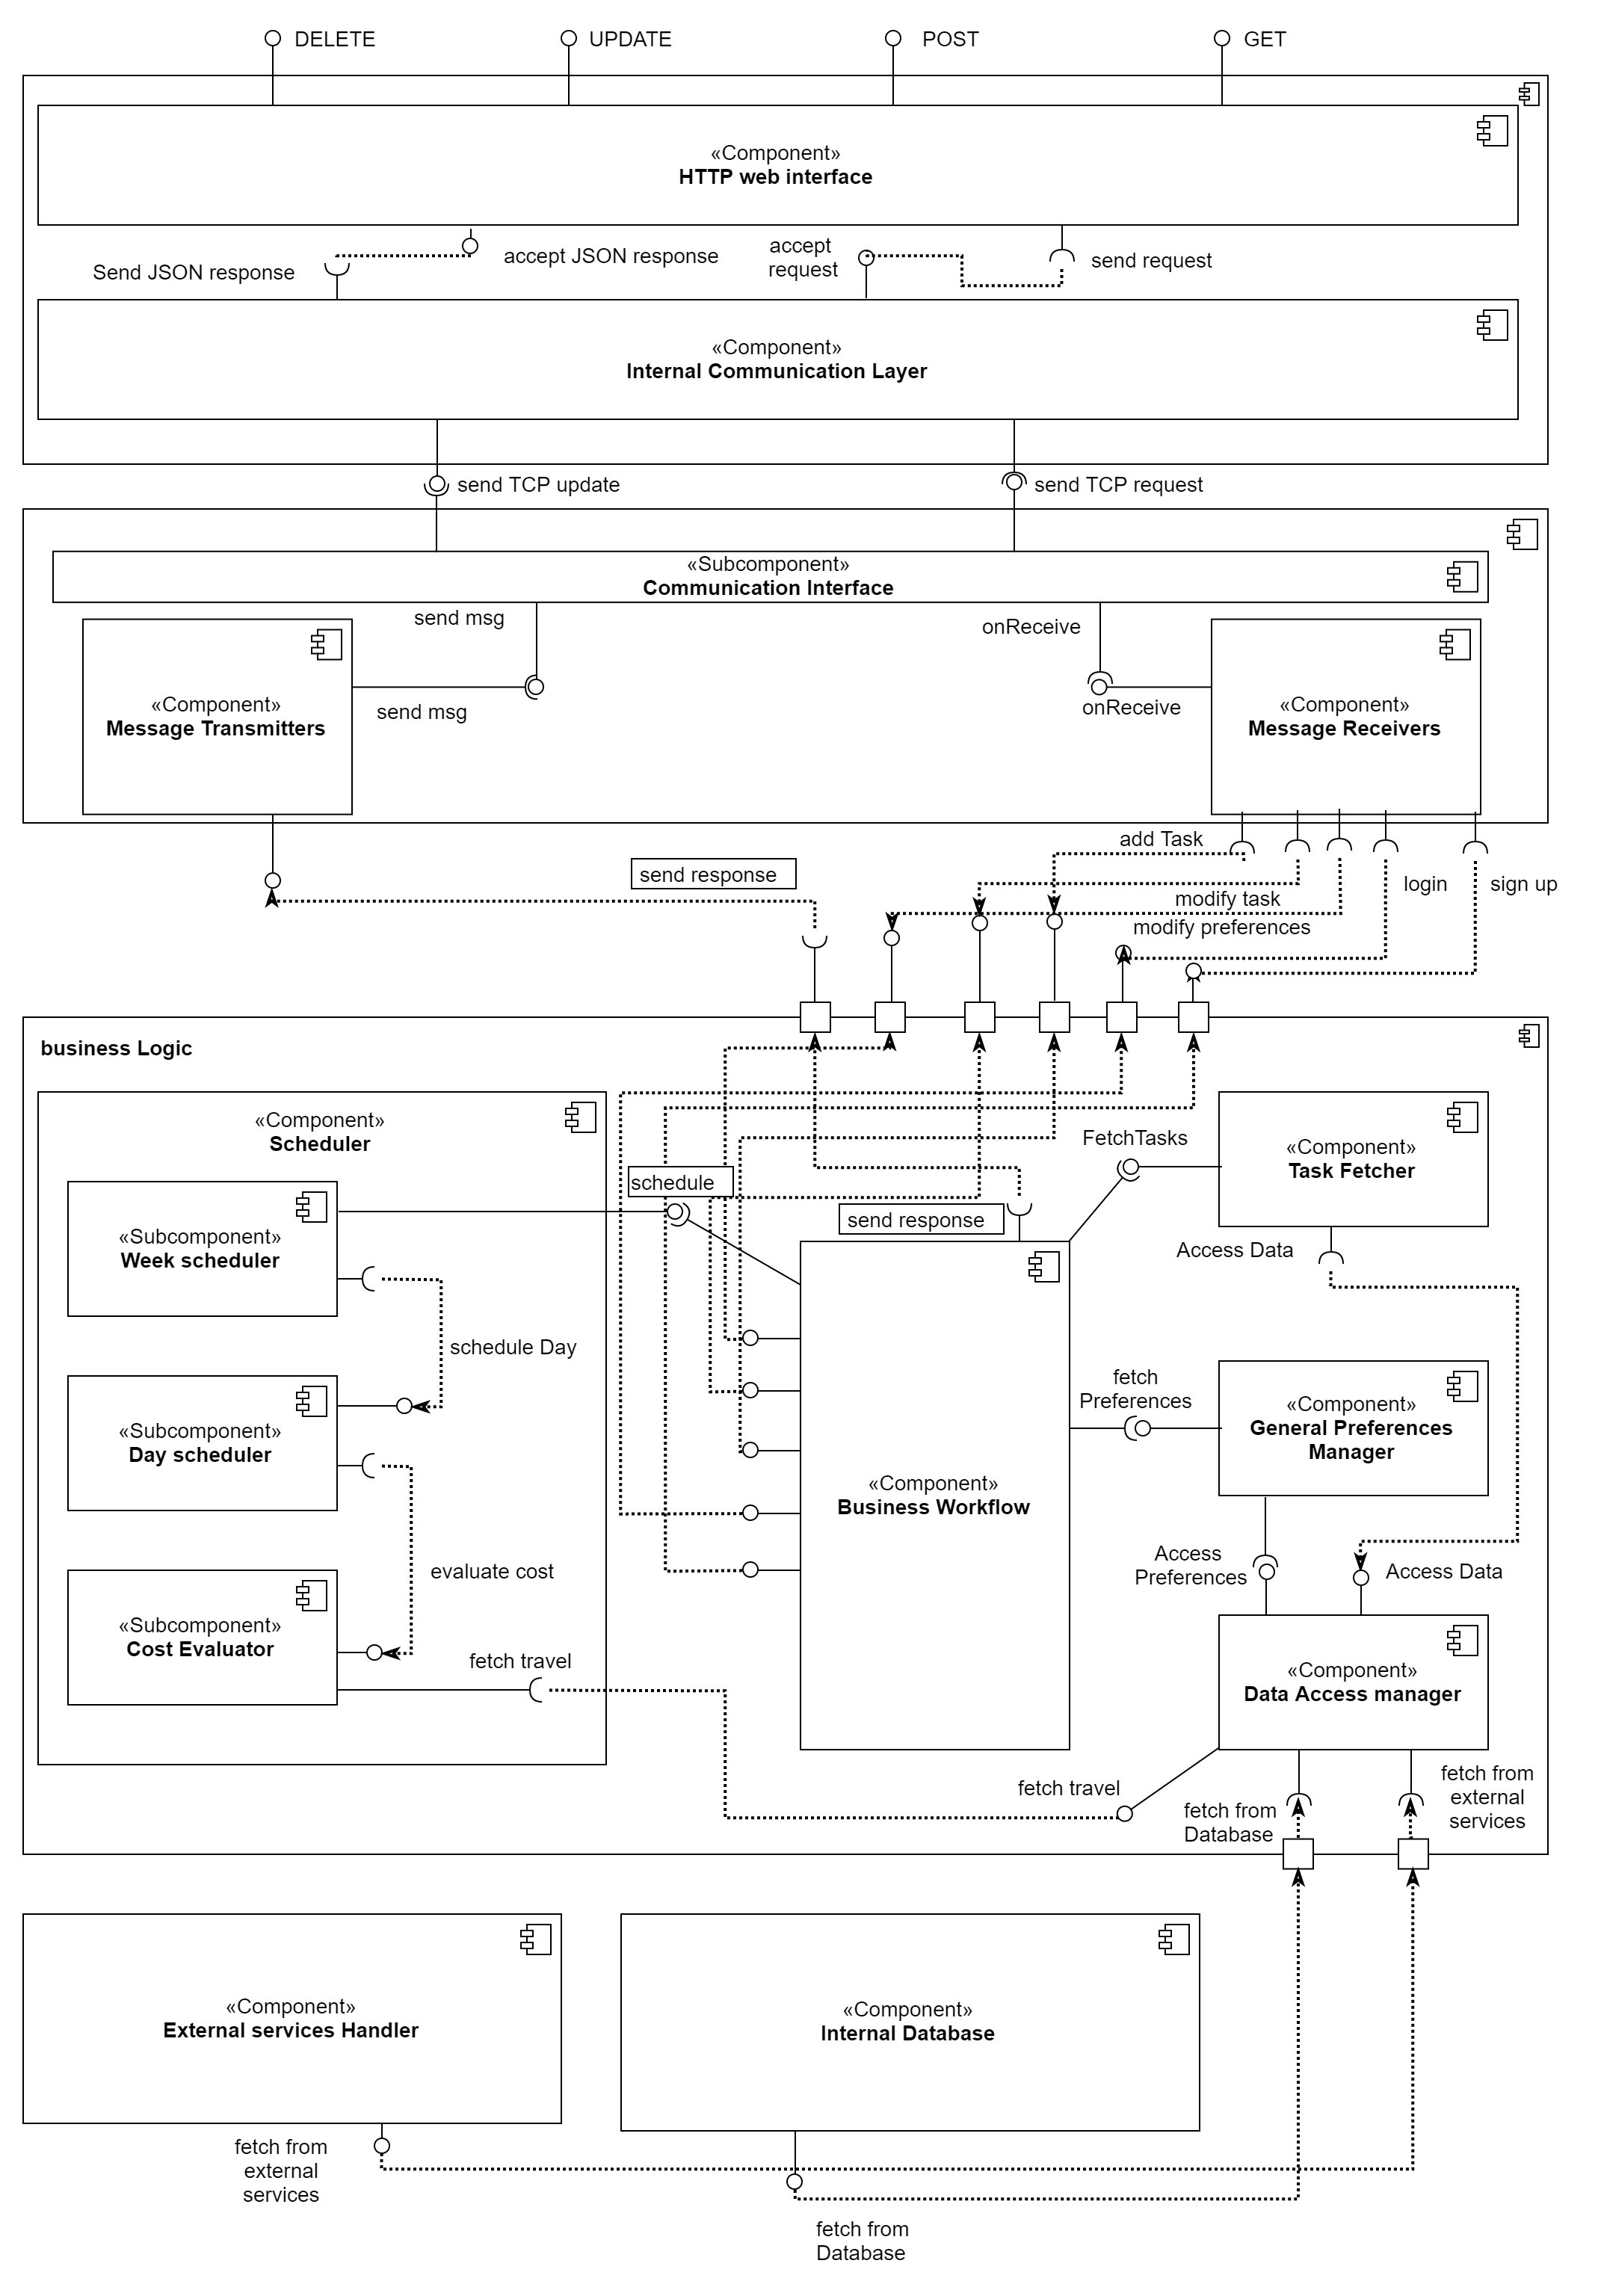
\includegraphics[scale=0.2]{Pictures/ComponentDiagram/componentDiagram.png}
    \caption{UML component diagram about back-end components}
\end{figure}
<<<<<<< HEAD
\newpage

\textbf{the Business Logic layer} is the main topic of this section. it can be divided in several different components which performs specific operations. here we present the main functionalities and the overall structure in terms of subcomponents, leaving the the subsection regarding the \emph{selected architectural styles and patterns} to describes how these subcomponents are meant to be implemented.

the business logic layer is composed by:
\begin{itemize}
    \item \textbf{the business workflow}: this is the component which takes in charge external requests and coordinates the activity of other business logic components, so allowing the core features of \emph{Travlendar+} to cooperate and produce a correct output. This means that the \emph{business components} interfaces itself with all the main components of our business logic architecture. nonetheless, he can also interface with the \emph{message tramitters} previously described, and is called by the \emph{message receivers} in order to properly handle messages from the frond-end.
    
    \item \textbf{the scheduler}: is the component in charge of schedule the user's task, which is the main core feature of the \emph{Travlendar+} software. It can be divided in other three subcomponents:
            \begin{itemize}
            
                \item \textit{the week scheduler}: this is the component that deals about dividing the weekly task who receives in input into the corresponding day, in order to be scheduled. the week scheduler takes care of both variable and flexible day tasks, where day fixed tasks need little computation.  to accomplish this goal we decide to use a stochastic approach, based on simple travel time estimations, leaving the heavy part of the scheduling algorithm to the day scheduler.
                
                \item \textit{the day scheduler}: this component is necessary to organize tasks between a single given day. it uses a particular version of the \emph{branch and bound} algorithm in order to return the optimal scheduling between the given day. it also relies on the \emph{cost evaluator} component in order to calculate the cost, in terms of money and time, of each solution.
                
                \item \textit{the cost evaluator}: this component takes care of calculating the cost of each travel solution. in order to do so, it needs to communicate with the \emph{data access manager} within the business logic, and so retrieve informations such as traffic or route options from the external services which the application relies on 
                
            \end{itemize}
            
    further description about how the scheduler works can be found in \emph{Chapter \ref{chapter:algo}}, which describes how the scheduling algorithm works.
    
    \item \textbf{the Data access manager}: this is the component in charge of extracting data from either external services and the \emph{Travlendar+} database. note that, in order to be as modular as possible, this component does not direclty interact with these data source, but relies on other minor components at data level. thus, his main goal is to build an high level representation of these data without having the other components to work about how to interpret. In this way we can claim this component as an \emph{adapter} between the business logic and the data layer.
    
    \item \textbf{the general preferences manager}: this component main goal is to manage the user preferences, as described in the \emph{Requirement analysis and specification document}, and then check whether certain solutions are admissible or not. thus, it needs to communicate both with the data access manager and the business workflow, in order to interpret "complex" preferences such as an \emph{eco friendly} profile in much more simple instructions about how to build the  
    schedule.
    
    \item \textbf{the Task fetcher}: as the other component, the main goal of the \emph{task fetcher} is either to create an high level representation of data from the data layer. in particular, the task fetcher needs to build the task entities using data from the access manager, from those extracting only the ones who are relevant to the scheduling, modifying them when needed and performing other similar operations.
\end{itemize}
=======
>>>>>>> ad258dd7c9a37861a484c05c0be22fc9761a519f

